%TODO: add LLVM-IR example/CFG picture, etc.

The LLVM project was started in 2000 by Chris Lattner, as a research project at the University of Illinois with the goal of providing a modern, \emph{Static Single Assignment} (SSA)-based compilation strategy capable of supporting both static and dynamic compilation of arbitrary programming languages. It was first released in 2003 and the project has grown rapidly since then. It has become popular amongst major companies, e.g. Google, Apple, and Sony, for its powerful multi-stage compilation strategy and outstanding extendability. LLVM is a collection of modular and reusable compiler and toolchain technologies. Generally, LLVM follows a 3-phase design, which is divided between a frontend, a code independent optimizer and a backend, illustrated in Figure \ref{fig:3phase_design}.

\begin{figure}[H]
\centering
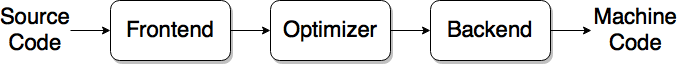
\includegraphics[width=.75\textwidth]{figures/3phase_design}%
\caption{3-phase design: frontend, optimizer and backend.}
\label{fig:3phase_design}
\end{figure}

%TODO: Reorder list: [IR, Lexical analysis, Syntax analysis, ]
\textbf{The frontend} is responsible for translating code of an arbitrary programming language into LLVM's \emph{Intermediate Representation} (IR) code. The LLVM instruction set represents a virtual architecture that captures the key operations of ordinary processors, but avoids machine specific constraints such as physical registers. Instead, it has an infinite amount of virtual registers in SSA form, which means that each virtual register is assigned only once and each use of a variable is dominated by that variable's definition. This simplifies the data flow optimizations because only a single definition can reach a particular use of a value, and to find that definition is trivial \cite{llvm_strategy}.

%\begin{lstlisting}[caption=Bundled instructions.,frame=tlrb]{ir_c}
%
%\end{lstlisting}

%TODO discuss of this example with phi should be in there? is it usefull? think not
%\captionof{lstlisting}{Fragment of code with a phi instruction.}
%\begin{center}
%\hspace{2px}\begin{minipage}{.475\textwidth}
%\lstset{style=customc}
%\begin{lstlisting}[caption=List of instructions.,frame=tlrb]
%\begin{lstlisting}[frame=tlrb]
%int foo(int a, int b)
%{
%  if (a > b)
%    return a;
%  else
%    return b;
%}
%
%
%
%
%
%
%<@\ @>
%\end{lstlisting}
%\end{minipage}\hfill
%\begin{minipage}{.475\textwidth}
%\lstset{style=customasm}
%%\begin{lstlisting}[caption=IR-code.,frame=tlrb]
%\begin{lstlisting}[breaklines, frame=tlrb]
%define i32 @foo(i32 %a, i32 %b) #0 {
%entry:
%  %cmp = icmp sgt i32 %a, %b
%  br i1 %cmp, label %if.then, label    %if.else
%if.then:
%  br label %return
%if.else:
%  br label %return
%return:
%  %retval.0 = phi i32 [ %a, %if.then ], [ %b, %if.else ]
%  ret i32 %retval.0
%}
%\end{lstlisting}
%%\vspace{1.9em}
%\end{minipage}
%\end{center}

%frontend talk, straight from the Dragon Book plz.
%introduce parser and lexical analysis and that it is kept in an AST, which will be translated as a final step to IR.
%Perhaps an example?
%TODO: rewrite first sentence in my own words.
Figure \ref{fig:frontend} gives an overview of a frontend. The main task of the lexical analyzer is to read the input characters of the source program, group them into luxemes, and produce as output a sequence of tokens. These tokens are used by the parser for syntax analysis, where it is verified that the sequence of tokens can be reconstructed according to the syntax of the input language. The parser reports any syntax errors during this process and should be able to recover from the error in order to continue processing the rest of the program. The parser constructs a parse tree, and the semantic analyzer uses this parse tree to check for consistency with the language definition. Type checking is also done during this stage, and the information is kept in a syntax tree. The result of these phases is an \emph{Abstract Syntax Tree} (AST) of the program, which can be translated into three-address IR code. %We will discuss LLVM's IR in more detail in Chapter \ref{sec:ir}

\begin{figure}[t]
\centering
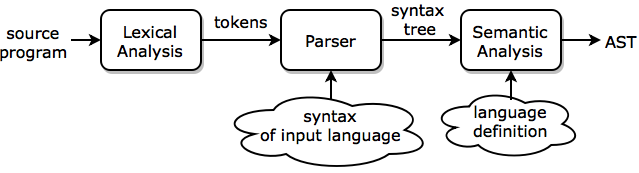
\includegraphics[width=\textwidth]{figures/frontend}%
\caption{Overview of the components that the frontend compromises.}
\label{fig:frontend}
\end{figure}

Listing \ref{lst:ir_code} shows an example C code where where we multiply two arguments and add them together to a third argument. On the right-hand part of this listing we can see the output that is generated by the front-end. Here we already have a notion of labels, similar to that of assembly code. The LLVM-IR code is in SSA form and consists of three-address operations. Here \emph{nsw} indicates that the result is undefined in case of an overflow.
%TODO BIG: add reference to 2.1, tell something about llvm's ir code representation, give examples, show phi node. 

\captionof{lstlisting}{Fragment of C code with corresponding LLVM-IR.}\label{lst:ir_code}
\begin{center}
\hspace{2px}\begin{minipage}{.475\textwidth}
\lstset{style=customc}
%\begin{lstlisting}[caption=List of instructions.,frame=tlrb]
\begin{lstlisting}[frame=tlrb]
int foo(int a, int b, int c)
{
  c += a*b;
  return c;
}

<@\ @>
\end{lstlisting}
\end{minipage}\hfill
\begin{minipage}{.475\textwidth}
\lstset{style=customasm}
%\begin{lstlisting}[caption=IR-code.,frame=tlrb]
\begin{lstlisting}[frame=tlrb]
define i32 @foo(i32 %a, i32 %b, 
                i32 %c) #0 {
entry:
  %mul = mul nsw i32 %b, %a
  %add = add nsw i32 %mul, %c
  ret i32 %add
}
\end{lstlisting}
%\vspace{1.9em}
\end{minipage}
\end{center}

% TODO: make graph to categorise optimizations on some criteria
\textbf{The optimizer} contains a collection of analysis and semantic-preserving transformations that can be used to optimize IR code. One of the advantages of LLVM is that when you build a new backend for any given processor architecture you immediately have access to all of these optimizations. Below we give some of these optimizations that are explained more detailed in the literature \cite[Chapter~9]{dragon_book}.%TODO: fix chapter in cite.
%TODO: add mem2reg
\begin{itemize}
\item \emph{Constant propagation:} computes for each point and each variable in the program, whether that variable has a unique constant value at that point. This can then be used to replace variable references with constant values.
\item \emph{Constant folding:} recognizes and evaluates constant expressions at compile time rather than runtime. For example, `$add\ 1+2$' can be replaced by `$3$'. Statements like `$add\ 1+2$' can be introduced by other optimizations, e.g. constant propagation. 
\item \emph{Common sub-expression elimination:} recognizes that the same expression appears in more than one place, and that performance can be improved by transforming the code such that the expression appears in one only place.
\item \emph{Copy propagation:} replaces each target of a copy statement with that of the copied value. For example, if we have a copy statement, $x = y$. Then the uses of $x$ can be replaced by $y$. Some optimizations require that this optimization is performed afterward to clean up, e.g. common sub-expression elimination requires this pass to run afterward. 
\item \emph{Dead code elimination:} removes code that does not affect the program's results. This avoids executing irrelevant operations and reduces the code size of a program.  
\item \emph{Loop invariant code motion:} aims at moving code that is independent of the loop iteration out of the loop body. It does this by moving the loop independent statement above the loop, saving it in a temporary variable, and use it in each iteration of the loop. Now the loop independent statement is computed only once instead of every iteration. 
\item \emph{Function inlining:} verifies whether inlining functions in its callees gives a performance benefit. If doing this would give a performance benefit, it replaces the call to the function with the function body. This optimization often is useful for small functions because it reduces the overhead that is introduced when a function call is made, e.g. storing frame pointer, storing function parameters and jump to the code to where the function is defined.     
\end{itemize}

\begin{figure}[b!]
\centering
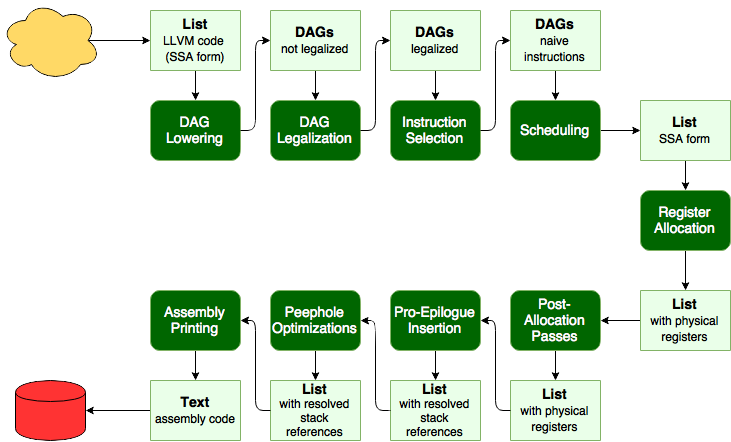
\includegraphics[width=\textwidth]{figures/code_generation_sequence}%
\caption{Code generation sequence, from LLVM code to assembly code.}
\label{fig:code_generation}
\end{figure}

%TODO: apply following namings: Instruction, Machine instruction, scheduled instruction in SSA form, schedule instruction not in SSA form.
\textbf{The backend} translates, according to a processor architecture, IR code to a target specific assembly language. It does this by going through a sequence of code generation stages, illustrated in Figure \ref{fig:code_generation}. The rectangular boxes indicate the data structure that is used by and produced by a given stage, and the name of each stage is denoted in a rectangular box with rounded corners. During this process, first, the IR code is lowered to a \emph{Directed Acyclic Graph} (DAG) in which each node represents an instruction. However, for some architectures, not all data types and instructions are supported. For this reason, the DAG is legalized to something that is supported by the target architecture. Instruction selection maps each of the nodes onto machine nodes, by matching patterns. %After that, the instruction selector maps the pattern of LLVM code into the target machine code and builds a new DAG whose nodes represents the target instructions.
Then we have a DAG consisting of only target specific machine instructions, in SSA form. Having naive machine instructions, the next step is to schedule them. We schedule the machine instructions according to the resource information of the target processor and assign each instruction to a specific cycle. 
%We will discuss scheduling in more detail in Chapter \ref{sec:scheduling}. 
Now the instructions are represented in a list rather than a DAG, but still in SSA form. The \emph{Register Allocator} (RA) then assigns physical registers to each of the virtual registers, now the list is not in SSA form. 
%We will discuss RA in more detail in Chapter \ref{sec:register_allocation}. 

The post-allocation pass can improve the schedule by taking physical registers and register pressure, that is known at this point, into account. After that, some epilogue and prologue code may be inserted, for example, saving/restoring the caller/callee registers and reserving/destroying of the function's stack frame. Peephole optimizations are target specific improvements to the generated code. These optimizations deal with very specific optimizations that can only be done at the end of the process. Finally, the assembly printer prints the generated code to a file.
%backend talk -> huuge



%\subsection{Instruction Scheduling}\label{sec:scheduling}
%After instruction selection, the program is represented in SSA form as a DAG. Each instruction is represented as a $MachineSDNode$ in a $MachineBasicBlock$. After scheduling has been performed, each instructions now is represented as a $MachineInstr$. 



%ach instruction is scheduleDuring instruction schdduling, each $MachineBasicBlock$ is scheduled by the scheduler and transformed into a $MachineInstr$. After this phase, instructions are represented as $MachineInstr$.

%\subsection{Register Allocation}\label{sec:register_allocation}
%Register allocation is executed during the code generation phase and consists of finding a mapping of a program with an unlimited number of virtual registers to a program with a limited number of physical registers.
%Examples, machine instrs on the left in SSA form, on the right with proper registers next to it.
%Introduce at least 

%TODO: 19 sept morning, Add examples of IR, CFG, Dominator tree ettc.
\subsection{Control Flow}\label{sec:control_flow_graph}
%\subsection{Representation of Code}
To analyze a code fragment, different representations can be explored. For instance, three-address IR code that is used by LLVM is conducive for further processing like optimizations and translations. Even further down the compilation line, we have assembly code, which is basically object code, but in human readable form. However, to analyze a fragment of code, we do not always need this much detail. Moreover, having this much detail, sometimes makes analysis more difficult. Control flow analysis is a code technique to analyze the control flow of a program. The control flow is expressed as a \emph{Control Flow Graph} (CFG), which is a more abstract representation of code that uses a graph notation to show all paths that can be traversed through a program during its execution.  
%TODO: Add cfg example with code left, cfg right

\begin{figure}[H]
\centering
\subfloat[C code fragment]{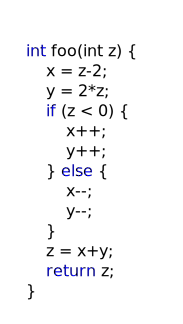
\includegraphics[width=.2\textwidth]{figures/cfg_fragment}%
\label{fig:cfg_fragment}}\quad\quad
\subfloat[CFG]{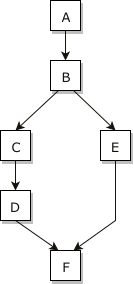
\includegraphics[width=.175\textwidth]{figures/cfg_fork_join}%
\label{fig:cfg_graph}}
\hfill
\caption{Example CFG with C code.}
\label{fig:cfg}
\end{figure}

In Figure \ref{fig:cfg_graph} we see a CFG for the code fragment in Figure \ref{fig:cfg_fragment}. In a CFG edges represent the control flow of the program and nodes represent basic blocks. A \emph{Basic Block} (BB) is a sequence of instructions with no branches, except for entering and leaving the basic block.
\\

%Another code representation that we would like to discuss here is a Dominator Tree (DomTree). Similar to a CFG, nodes represent BBs, but edges represent a dominator relationship. For two nodes $A$ and $B$, we say that $A$ dominates $B$, if all paths to $B$ go through $A$.

%TODO: add example CFG with corresponding DomTree

\subsection{Data Dependencies and Spilling}\label{sec:data_dependencies}
%\subsection{Scheduling Constraints}\label{sec:scheduling_and_ra}
%As we have seen above,
From a compilers perspective, certain operations address memory locations. A \emph{store} operation accesses the memory to put the value of a register into memory at a certain location, addressable by its address. On the other hand, \emph{load} operations load a value from memory at a certain location and puts that value in a register. These kind of operations are called memory operations. Other operations calculate a value and stores the result in a register. Operations that store the result in a register, or load a value from memory into a register, actually define that register. An example is given in the following code fragment:

%\lstset{style=customasm}
\begin{lstlisting}
lw  r2, r0, 4   # load from memory at location 0x4
lw  r3, r0, 5   # load from memory at location 0x5
mul r3, r3, r2  # define r3 with r3 = r3 * r3
sw  r3, r0, 2   # store result at location 0x2
\end{lstlisting}

Before scheduling and register allocation, the sequence of instructions contain an unlimited number of virtual registers and the instructions are in a DAG that preserves all control flow and data dependencies. Data dependencies are ordering constraints that influence the order of execution. Typically, there are three kinds of data dependencies \cite{data_dependece}:
\begin{enumerate}
\item There is a Read-after-Write (RaW) dependency, also called a \emph{flow dependency} from operation $a$ to operation $b$ if $a$ defines a register that may be used by $b$.
\item  There is a Write-after-Read (WaR) dependency, also called an \emph{anti-dependency} if for operations $a$ and $b$ when $a$ uses a register that is redefined by $b$. 
\item There is a Write-after-Write (WaW) dependency, or \emph{output dependency} from operation $a$ to operation $b$, if $a$ defines a register that is redefined by $b$.
\end{enumerate} 

Flow dependencies are also known as \emph{true dependencies} and anti and output dependencies as \emph{false dependencies}, introduced by scheduling or register allocation. While in SSA form, each variable is defined exactly once, therefore, we have only true dependencies in that form. After scheduling and register allocation, where we assign physical registers to each virtual register, we may assign one physical register to multiple virtual registers, which is illustrated in Listing \ref{lst:ra_example}. This process introduces false dependencies and can often be resolved with renaming techniques \cite{tta_codegen,renaming}.

\captionof{lstlisting}{Redefining physical registers by assigning them to multiple virtual registers.}
\begin{center}
%TODO: include a data dependency graph for the example below
\hspace{2px}\begin{minipage}[t]{.475\textwidth}
\begin{lstlisting}[frame=tlrb]
mul %v1, %src1, %src2
add %v2, %1,    %sum
mul %v3, %src3, %src4
add %v4, %v2,   v3
\end{lstlisting}
\end{minipage}\hfill
\begin{minipage}[t]{.475\textwidth}
\begin{lstlisting}[frame=tlrb]
mul r1, r5, r6
add r2, r1, r21
mul <@\hspace{1px}\textcolor{red!70!black}{r1}\hspace{1px}@>, r7, r8  # redefines r1
add <@\hspace{1px}\textcolor{red!70!black}{r2}\hspace{1px}@>, r2, r1  # redefines r2
\end{lstlisting}
\end{minipage}
\label{lst:ra_example}
\end{center}

%\lstset{style=customasm}
%\begin{center}
%\begin{minipage}{\linewidth}
%      \centering
%      \begin{minipage}{0.45\linewidth}
%          \begin{lstlisting}[frame=tlrb]
%(a) lw  r2, r5, 4
%(b) lw  r3, r6, 6
%(c) mul r3, r3, r2
%(d) lw  r4, r7, 0
%(e) add r4, r3, r4
%(f) sw  r4, r11, 0
%\end{lstlisting}
%          \captionof{subfigure}{Assembly code}
%          \label{fig:ddg_fragment}
%      \end{minipage}
%      \begin{minipage}{0.45\linewidth}
%          \begin{figure}[H]
%          \centering
%              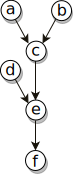
\includegraphics[width=.2\textwidth]{figures/ddg}%
%          \end{figure}
%          \captionof{subfigure}{DDG}
%          \label{fig:ddg_graph}
%      \end{minipage}
%\captionof{figure}{Example DDG with corresponding assembly code.}
%\label{fig:ddg}
%\end{minipage}
%\end{center}
%TODO: add more abstractions, also include dominator tree
Figure \ref{fig:ddg_graph} shows a data dependence graph corresponding to the code fragment in Figure \ref{fig:ddg_fragment}. In a data dependence graph nodes represent operations and the edges correspond to data dependencies.

%========= Store listing box =====
\newsavebox{\ddgfragmentlst}
\begin{lrbox}{\ddgfragmentlst}
  \begin{lstlisting}
(a) lw  r2, r5,  4
(b) lw  r3, r6,  6
(c) mul r3, r3, r2
(d) lw  r4, r7,  0
(e) add r4, r3, r4
(f) sw  r4, r11, 0
  \end{lstlisting}
\end{lrbox}

\begin{figure}[H]
  \centering
  \subfloat[Assembly fragment]{%
%    \usebox{\ddgfragmentlst}\label{fig:ddg_fragment}
   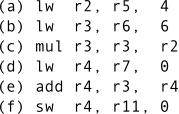
\includegraphics[width=.25\textwidth]{figures/ddg_fragment}\label{fig:ddg_fragment}
  } \quad\quad%\hfill%\hspace{35px}
  \subfloat[DDG]{%
   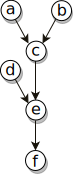
\includegraphics[width=.1\textwidth]{figures/ddg}\label{fig:ddg_graph}
  }
  \caption{Example DDG with corresponding assembly code.}
  \label{fig:ddg}
\end{figure}


%new TODO: add live interval analysis information or theory!!!
%TODO: add sentence in between
Sometimes there are not enough registers available to allocate physical rezgisters to all virtual registers because there are only a limited number of physical registers available. When the compiler runs out of registers to allocate, \emph{spilling} may be necessary to free one or more registers by storing them on the stack. Consequently, it is required to retrieve them from the stack just before they are used.

%TODO: add illustration of spilling?

%todo add theory, graph coloring on ddg graph.


%TODO: add control flow dependecy explanation, optionally from Code Generation for TTAs p.
%TODO: play with widths to get nicely in teh middle of the page.
%\lstset{style=customc}
%\begin{center}
%\begin{minipage}{\linewidth}
%\centering
%\begin{minipage}{0.2\linewidth}
%\begin{lstlisting}
%
%int foo(int z) {
%  x = z-2;
%  y = 2*z;
%  if (z < 0) {
%    x++;
%    y++;
%  } else {
%    x--;
%    y--;
%  }
%  z = x+y;
%  return z;
%}
%\end{lstlisting}
%\end{minipage}
%\hspace{0.05\linewidth}
%\begin{minipage}{0.4\linewidth}
%\begin{figure}[H]
%\centering
%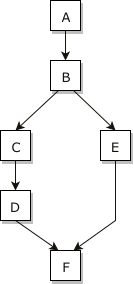
\includegraphics[width=.35\textwidth]{figures/cfg_fork_join}%
%\end{figure}
%\end{minipage}
%\captionof{figure}{A fragment of C code with a CFG.}
%\label{fig:cfg}
%\end{minipage}
%\end{center}

%TODO: insert general RA algorithms and heuristics. Graph colouring, and use this reference \cite{ra}.
%There are multiple register allocators available in LLVM, e.g. basic, fast, greedy and Partitioned Boolean Quadratic Problem (PBQP) register allocation. PBQP is a nearly optimal approach that does register allocation in phases, i.e. spilling, register assignment and copy coalescing. After spilling, RA can be done in polynomial time, but copy coalescing is NP-complete \cite{pbqp}. The other three register allocators are linear scan based algorithms that use heuristics and visit live ranges in order, although it is possible to implement a custom register allocator.
%TODO: decide to add or not to add.

%TODO: insert scheduling talk, including algorithms, heuristics and LLVMs available schedulers.
%TODO: move to later.
%A common problem in compilers is the ordering in which to do scheduling and register allocation. If registers are allocated before scheduling, the resulting code tends to have many storage dependencies that limit code scheduling. On the other hand, if the code is scheduled before register allocation, the schedule created may require so many registers that register spilling is required, which may negate the advantages of instruction-level parallelism (ILP) \cite[Chapter~10.2.4]{dragon_book}. Whether to do register allocation first, or scheduling first, or to address these problems at the same time is often referred to as, phase-ordering problem. 

%In general, you can solve scheduling exactly using algorithms, e.g. integer programming or constraint programming, or one can solve the problem, but without guaranteeing that an optimal solution is found using heuristics. With LLVM there are two main schedulers, i.e. list scheduler and Machine Instruction (MI) scheduler that use heuristics to find a solution, although it is possible to implement a custom scheduler for an architecture at hand. 

%TODO: add basic introduction to bypassing, from presentation.